\chapter{Il package Navigation}
Il \emph{package} \texttt{it.polito.Navigation} contiene le classi deputate a gestire i movimenti del Robot sulla scacchiera.\\
In particolare sono stati progettati due controllori: \texttt{CheckersNavigator} e \texttt{ArmController} che sono responsabili rispettivamente della navigazione nelle due direzioni orizzontali e in quella verticale.\\
Di seguito si entrer� nel dettaglio delle implementazioni delle classi sopra citate e dei relativi helper.
\section{La classe LashMotor}
\section{L'interfaccia  CheckersNavigator}
Questa interfaccia astrae le funzionalit� di movimento bidimensionale sulla scacchiera 8x8; i metodi pi� importanti sono:

\begin{lstlisting}
/** Ritorna la posizione X [0; 7] */
public int getX(); 
/** Ritorna la posizione Y [0; 7] */
public int getY(); 
/** Muove il braccio sulla casella (X, Y) */
public void goTo(int newX, int newY) throws NotCalibratedException; 
/** Muove il braccio sulla casella "base" */
public void goHome() throws NotCalibratedException; 
/** Modifica la velocit� dei motori */
public void setSpeed(int speedA, int speedB);
/** Effettua la calibrazione */
public void calibrate();
\end{lstlisting}
Si noti come i metodi che comportano un movimento non possano essere eseguiti se prima non � stata effettuata la calibrazione (eccezione \texttt{NotCalibratedException}).\\
Esamineremo ora le implementazioni che sono state progettate per questa interfaccia.

\subsection{La classe SimpleNavigator}
Questa prima implementazione si basa su un mapping statico di tutte le caselle relativo ad un punto iniziale su cui il Robot tenta di posizionarsi in fase di calibrazione.

\paragraph{Calibrazione}
Il Robot, per come � costruito, pu� ruotare il suo braccio agendo sul motore B, o pu� spostarlo avanti e indietro agendo sul motore A.\\
Il primo metodo di calibrazione che � stato pensato � pertanto semplicemente mirato a portare il braccio in una posizione nota (punto rosso in Figura \ref{simpleNavigatorGrid}), in modo da poter usare offset predeterminati (relativi ad essa) per spostarlo su tutte le altre caselle. \\
\begin{figure}[htbp]
\begin{center}
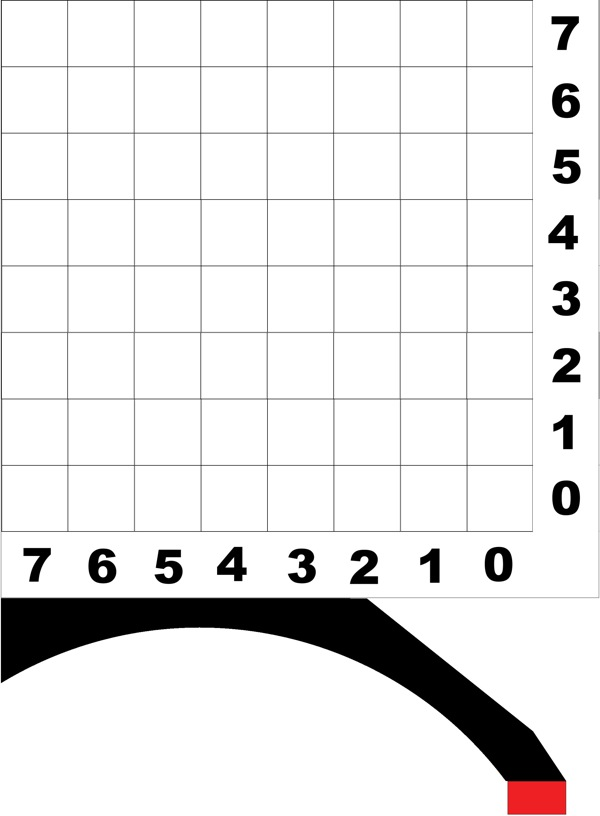
\includegraphics{img/simpleNavigatorGrid.jpg}
\caption{Scacchiera SimpleNavigator \label{simpleNavigatorGrid}}
\end{center}
\end{figure}
Il metodo \texttt{calibrate()} non fa altro che ruotare il braccio verso destra finch� il sensore di colore montato su di esso non rileva il colore rosso, a quel punto recupera eventuali giochi dei motori e azzera i contatori di distanza angolare in essi contenuti.

\paragraph{Navigazione}
Gli angoli di destinazione cui vengono fatti ruotare i motori sono calcolati semplicemente come\footnote{X e Y sono rispettivamente le  coordinate di ascissa e di ordinata delle caselle}: 
\begin{lstlisting}
destAngleA = offA+posy[newY]+dely[newX];
destAngleB = offB+posx[newX];
\end{lstlisting}
I vettori \texttt{posx} e \texttt{posy} definiscono l'offset in funzione delle rispettive coordinate; il vettore \texttt{dely} contiene le correzioni da effettuare sull'asse y in funzione della coordinata x, in modo da recuperare gli scostamenti in verticale dati dal fatto che il braccio si muove su un arco di circonferenza.\\
Le costanti \texttt{offA} e \texttt{offB} definiscono invece l'offset necessario a portare il braccio sulla casella (5,0) che costituiva il punto pi� comodo cui riferire la taratura di tutte le altre caselle.

\subsection{La classe MathNavigator}
\paragraph{Calibrazione}
\paragraph{Navigazione}

\section{La classe ArmController}
